\section{Archive and Implementation Details}
\label{sec:archive}

\paragraph{Source of the technical description.}
The principal implementation is the v2 notebook, while v0 documents architectural and sampling development. The repository preserves both original files in its notebooks directory, together with their SHA-256 hashes. The description in this manuscript was obtained by inspecting code and saved outputs. No notebook training or generation cell was executed to prepare this draft. The separate NVD notebooks are not evidence for the ReGAE results.

\paragraph{Stage boundaries.}
The v2 configuration jointly trains the image encoder and decoder, then constructs latent maps for the Gencoder. The latter is a separately trained instance of the decoder family with 256 input/output channels and no external conditioning code. The image decoder uses three input/output channels and latent conditioning. Shared architecture thus refers to the computational construction, not tied weights. The patch-relative positional parameters do not encode global source-image coordinates.

\paragraph{Optimization and reproducibility.}
The recorded environment reports PyTorch 2.2.2 with CUDA 12.1, and the code sets a random seed of 4202. These facts do not specify the original GPU, elapsed training time, or complete software environment. The archive contains configured training loops and saved displays, but no complete execution log establishing every historical state. In v2, the Gencoder loop computes a decaying learning rate but assigns it to the AE optimizer, leaving the Gencoder optimizer unchanged by that schedule. This is preserved as a historical qualification rather than silently corrected. Exact reproduction should distinguish a faithful historical configuration from a cleaned implementation.

\paragraph{Exploratory sampling in v0.}
The earlier notebook includes source-code reconstruction, latent generation, random overlapping patch updates, repeated local refinement, and shifted raster sweeps. Some updates protect previously completed pixels or use update-budget masks. Their motivation includes an analogy to wave-function-collapse-style synthesis. The cells do not implement a documented entropy-ranked constraint-propagation algorithm, and their current channel and conditioning assumptions are not mutually consistent with all retained network definitions. We therefore avoid presenting them as a verified benchmark of sampling strategies. The later v2 synchronous overlap average is specified explicitly in Eq.~\eqref{eq:regae-overlap-update}.

\paragraph{Extent of a latent window.}
The decoder tiles $32\times32$ generated image patches into a $1024\times1024$ macro-image. The source crops used to build a corresponding training window are positioned by the rounded lattice in Eq.~\eqref{eq:regae-grid-origins}, rather than exactly 32 pixels apart. ``Megapixel window'' consequently describes the decoded tile extent; it does not assert that all sampled training windows form an exact, gap-free partition of the source image.

\paragraph{Visual evidence to add from existing runs.}
The most informative additions would be a source region alongside its patch-code reconstruction, a spatially coherent Gencoder sample, and a short sequence showing a typical trajectory and a reported jump. Each should identify its checkpoint, sampler configuration, and whether its RGB rendering uses fresh noise. The unstable exponential-gate example cannot currently be illustrated from an original recording and should remain identified as an anecdote. This list specifies documentation needs, not new experiments or figures that already exist in this draft.

\section{Storage Accounting for the Proof of Concept}
\label{sec:storage}

The stored parameter counts are 4,673,752 for the encoder, 50,986,296 for the conditional image denoiser, and 85,479,680 for the Gencoder. These counts describe this implementation, not a required model size. Table~\ref{tab:storage} calculates uncompressed payloads in decimal megabytes. A code grid alone does not specify a complete codec for the image, including its boundary conventions and reconstruction distortion.

\begin{table}[t]
  \centering
  \small
  \setlength{\tabcolsep}{5pt}
  \begin{tabular}{lr}
    \toprule
    Representation or parameter payload & MB \\
    \midrule
    Source RGB array, 8 bits per channel & 710.45 \\
    One $419\times551\times256$ grid, FP32 & 236.41 \\
    Image encoder and denoiser, FP32 & 222.64 \\
    Gencoder, FP32 & 341.92 \\
    Image denoiser plus one grid, FP32 & 440.36 \\
    AE and Gencoder parameters, FP32 & 564.56 \\
    \bottomrule
  \end{tabular}
  \caption{Calculated uncompressed payloads for the Pandora setup. Rows describe different accounting choices, not interchangeable complete codecs. Optimizer state and file overhead are excluded. The four shifted training grids occupy approximately 945.64 MB in FP32.}
  \label{tab:storage}
\end{table}

AMSGrad stores three moment-related tensors per parameter in addition to the weights. Including these tensors in FP32 can bring training checkpoints near the author's recalled 0.89 GB for the AE and 1.4 GB for the Gencoder. This is an inference from the optimizer and parameter counts, not a measurement of the unavailable checkpoint files. A storage comparison with JPEG or another codec would also need quantization, coding, model costs, and matched reconstruction distortion.

\section{Preserved Training Plots}
\label{sec:traces}
The plots reproduce unchanged PNGs from the archived v2 outputs. Their horizontal axes count optimizer updates despite the inherited ``epoch'' label. Vertical values are square roots of different training objectives and are not directly comparable.

\begin{figure*}[t]
  \centering
  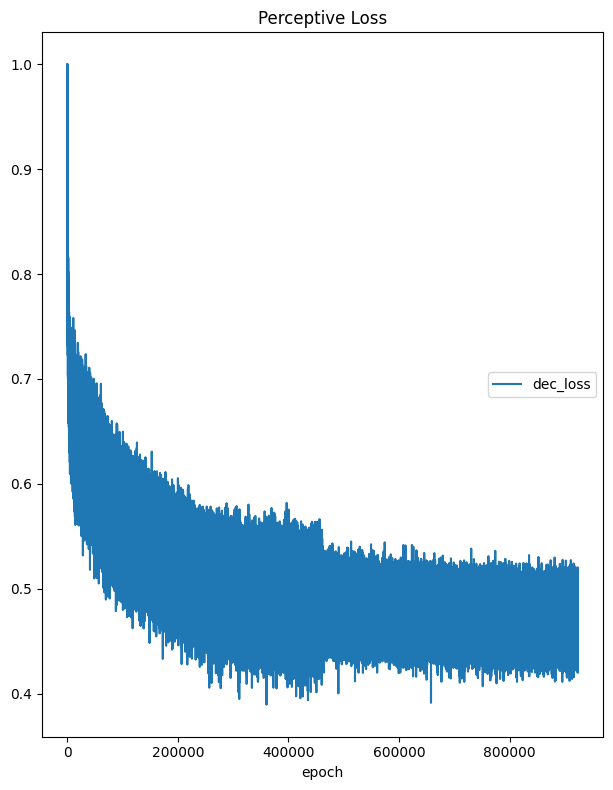
\includegraphics[width=0.86\textwidth]{figures/ae-training.png}
  \caption{Saved image-autoencoder training display (v2, code cell 39 under zero-based notebook indexing). The summary reports minimum 0.389, current 0.450, and maximum 1.000; the history was clipped to $[0,1]$ for plotting. The displayed quantity is the square root of the VGG feature $L_1$ loss. The history supports optimization of the training objective, not a held-out quality estimate.}
  \label{fig:ae-trace}
\end{figure*}

\begin{figure*}[t]
  \centering
  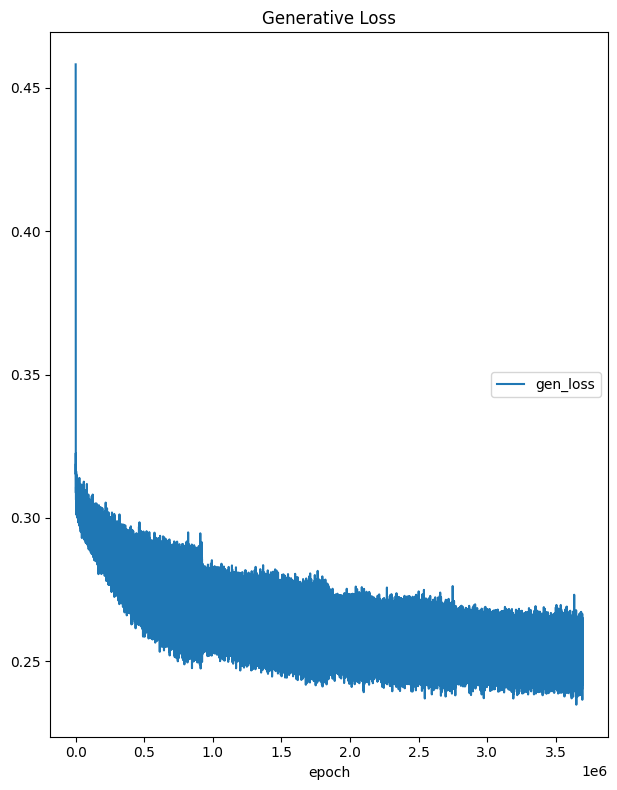
\includegraphics[width=0.86\textwidth]{figures/gencoder-training.png}
  \caption{Saved Gencoder training display (v2, code cell 46 under zero-based notebook indexing). The summary reports minimum 0.235, current 0.252, and maximum 0.458. The displayed quantity is the square root of the latent $L_1$ prediction loss. No new training was run to produce this figure.}
  \label{fig:gencoder-trace}
\end{figure*}
